\documentclass[11pt,letterpaper]{article}

\usepackage[utf8]{inputenc}
\usepackage{amsmath}
\usepackage{amsfonts}
\usepackage{amssymb}
\usepackage{fancyhdr}
\usepackage{graphicx}
\usepackage{listings}% http://ctan.org/pkg/listings
\usepackage{xcolor}
\usepackage{hyperref}
\usepackage{pdfpages}

\definecolor{codegreen}{rgb}{0,0.6,0}
\definecolor{codegray}{rgb}{0.5,0.5,0.5}
\definecolor{codepurple}{rgb}{0.58,0,0.82}
\definecolor{backcolour}{rgb}{0.95,0.95,0.92}
\lstdefinestyle{mystyle}{
    backgroundcolor=\color{backcolour},   
    commentstyle=\color{codegreen},
    keywordstyle=\color{magenta},
    numberstyle=\tiny\color{codegray},
    stringstyle=\color{codepurple},
    basicstyle=\ttfamily\footnotesize,
    breakatwhitespace=false,         
    breaklines=true,                 
    captionpos=b,                    
    keepspaces=true,                 
    numbers=left,                    
    numbersep=5pt,                  
    showspaces=false,                
    showstringspaces=false,
    showtabs=false,
    tabsize=2
}

\hypersetup{
    colorlinks=true,
    linkcolor=blue,
    filecolor=magenta,      
    urlcolor=cyan,
}

\lstset{style=mystyle}

\pagestyle{fancy}
\fancyhf{}
\lhead{\footnotesize{Design Document: Persistant MT rpcserver}}
\rhead{\footnotesize{Perry David Ralston Jr. CruzID: pdralsto}}
\cfoot{\footnotesize{Page \thepage}}


\title{Design Document\\Persistant Multi-Threaded RPCServer}
\author{Perry David Ralston Jr.\\ CruzID: pdralsto}

\begin{document}
\maketitle
\thispagestyle{fancy}
\section{Goals}
\begin{enumerate}
\item Fix the bugs from asignment 2
\item Support synchronized storing of values or variable names in key/value store
\item Support recursive name resolution to a specified max depth
\item Support large scalability
\item Key-Value store will be persistant across instantiations of the server
\end{enumerate}

\section{Syncronized Hashtable}
The hashtable defined below utilizes the djb2 hashing function, sourced from http://www.cse.yorku.ca/$\sim$oz/hash.html on 11/23/2020. It supports these public functions:\\
\begin{tabular}{|c|c|c|}
\hline 
insert & remove & lookup \\ 
\hline 
clear & dump & load \\ 
\hline 
acquire & \multicolumn{2}{c|}{release} \\ 
\hline 
\end{tabular} 

\vspace{.5cm} Data is stored as a Singly-Linked List of Node objects, detailed below. The hash table is wrapped by an inherited class, SyncHash, that adds index level synchronization to the table. The syncronization is managed using a parallel array of mutexes and all of the functions use calls to acquire and release to change the states of them.

\subsection{Node Structure and Functions}

Nodes are structured as a key value pair with a pointer to the next node in the list. Nodes are inserted into the hash table by hashing their key to acquire the index for the list that they will be inserted into. Nodes are instantiated with their next pointers set to null. The data of the node is a union type int64\_t and char*. This allows for the nodes to store either a variable name or a numeric value, supporting recursive name resolution. See diagram below.

\begin{center}
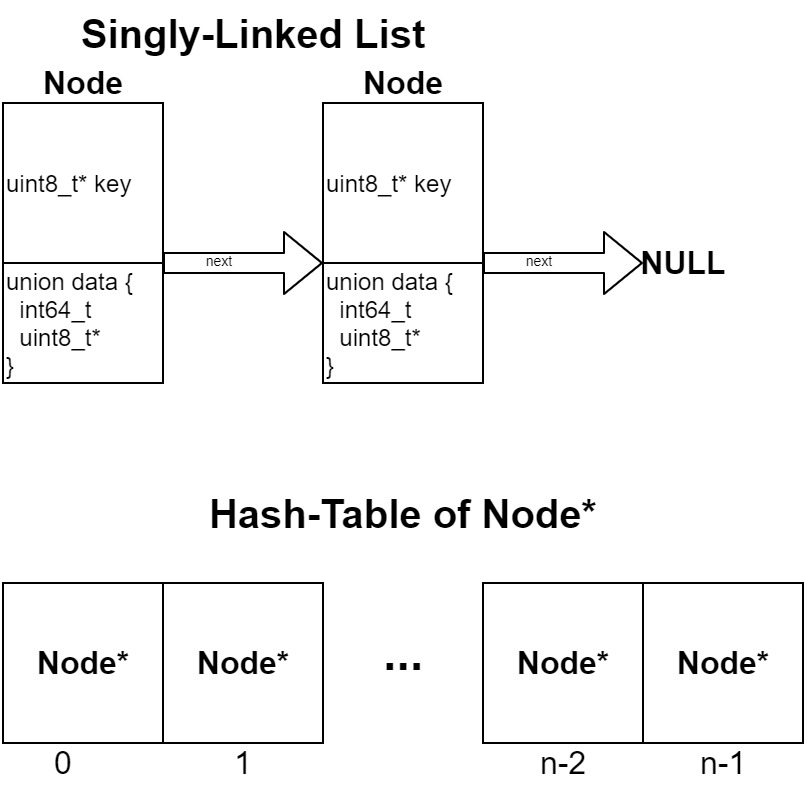
\includegraphics[scale=.4]{resources/node.jpg}
\end{center}
\pagebreak

\subsection{Hash Table Functions}
\begin{center}
\lstinputlisting[language=Python, frame=single]{resources/hashing_function}
\textbf{\footnotesize{Hashing Function}}
\end{center}
\pagebreak
Acquire and release supports two different public interfaces, single and list. The list
version acquires locks in index order to avoid dead lock.
\begin{center}
\lstinputlisting[language=Python, frame=single]{resources/acquire}
\textbf{\footnotesize{Acquire}}
\end{center}
\begin{center}
\lstinputlisting[language=Python, frame=single]{resources/acquire-list}
\textbf{\footnotesize{Acquire (list)}}
\end{center}
\begin{center}
\lstinputlisting[language=Python, frame=single]{resources/release}
\textbf{\footnotesize{Release}}
\end{center}
\begin{center}
\lstinputlisting[language=Python, frame=single]{resources/release-list}
\textbf{\footnotesize{Release (List)}}
\end{center}
\begin{center}
\lstinputlisting[language=Python, frame=single]{resources/insert}
\textbf{\footnotesize{Insert}}
\end{center}
\begin{center}
\lstinputlisting[language=Python, frame=single]{resources/delete}
\textbf{\footnotesize{Remove}}
\end{center}
\begin{center}
\lstinputlisting[language=Python, frame=single]{resources/lookup}
\textbf{\footnotesize{Lookup}}
\end{center}
\begin{center}
\lstinputlisting[language=Python, frame=single]{resources/clear}
\textbf{\footnotesize{Clear}}
\end{center}
\begin{center}
\lstinputlisting[language=Python, frame=single]{resources/dump}
\textbf{\footnotesize{Dump}}
\end{center}
\begin{center}
\lstinputlisting[language=Python, frame=single]{resources/load}
\textbf{\footnotesize{Load}}
\end{center}

\section{Multi-Threading}

In the previous rpcserver, request handling was limited to a single request at a time. Using the shared hash table described above and the pthread library, this rpcserver will have the ability to servce -N clients at the same time. -N is a command line argument that denotes the number of threads that the server should initially service. The default N value is 4. To achieve this, a structure will be created to house the thread references and act as a means of communication between the dispatch thread and the worker threads. The over all design is pictured below:
\begin{center}
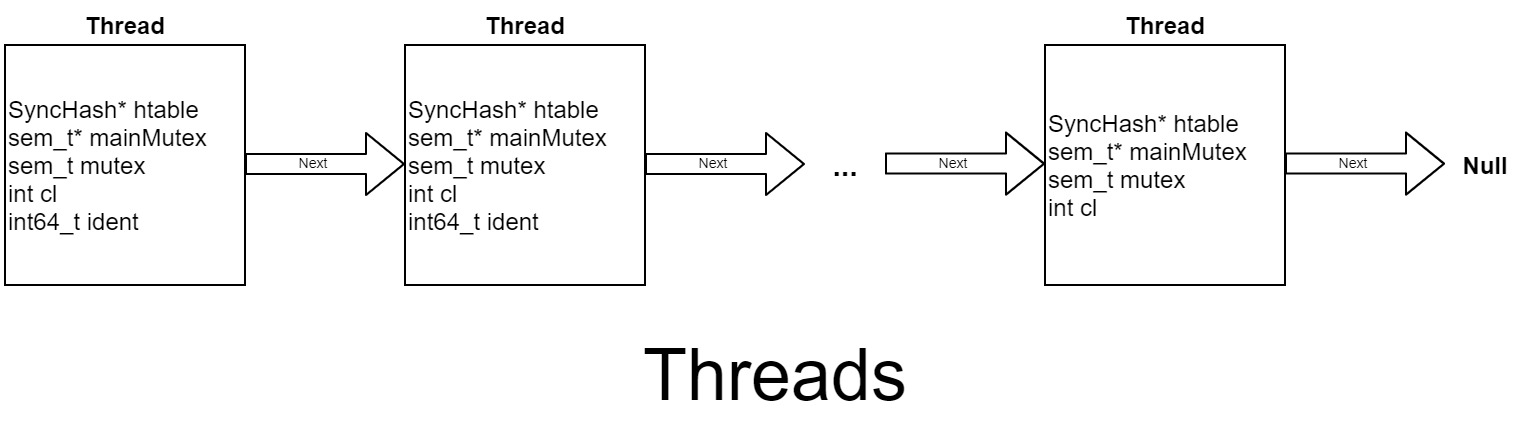
\includegraphics[scale=.25]{resources/threads.jpg}
\end{center}

The instructions for request handling are moved into a new function, process, that recieves a Thread\& as an argument. The Thread type is shown above and the members are used by the process function in order to facilitate synchronization of the access to the hashtable as well as retrieving and responding to the request from the client.

\begin{center}
\lstinputlisting[language=Python, frame=single]{resources/process}
\textbf{\footnotesize{Process}}
\end{center}

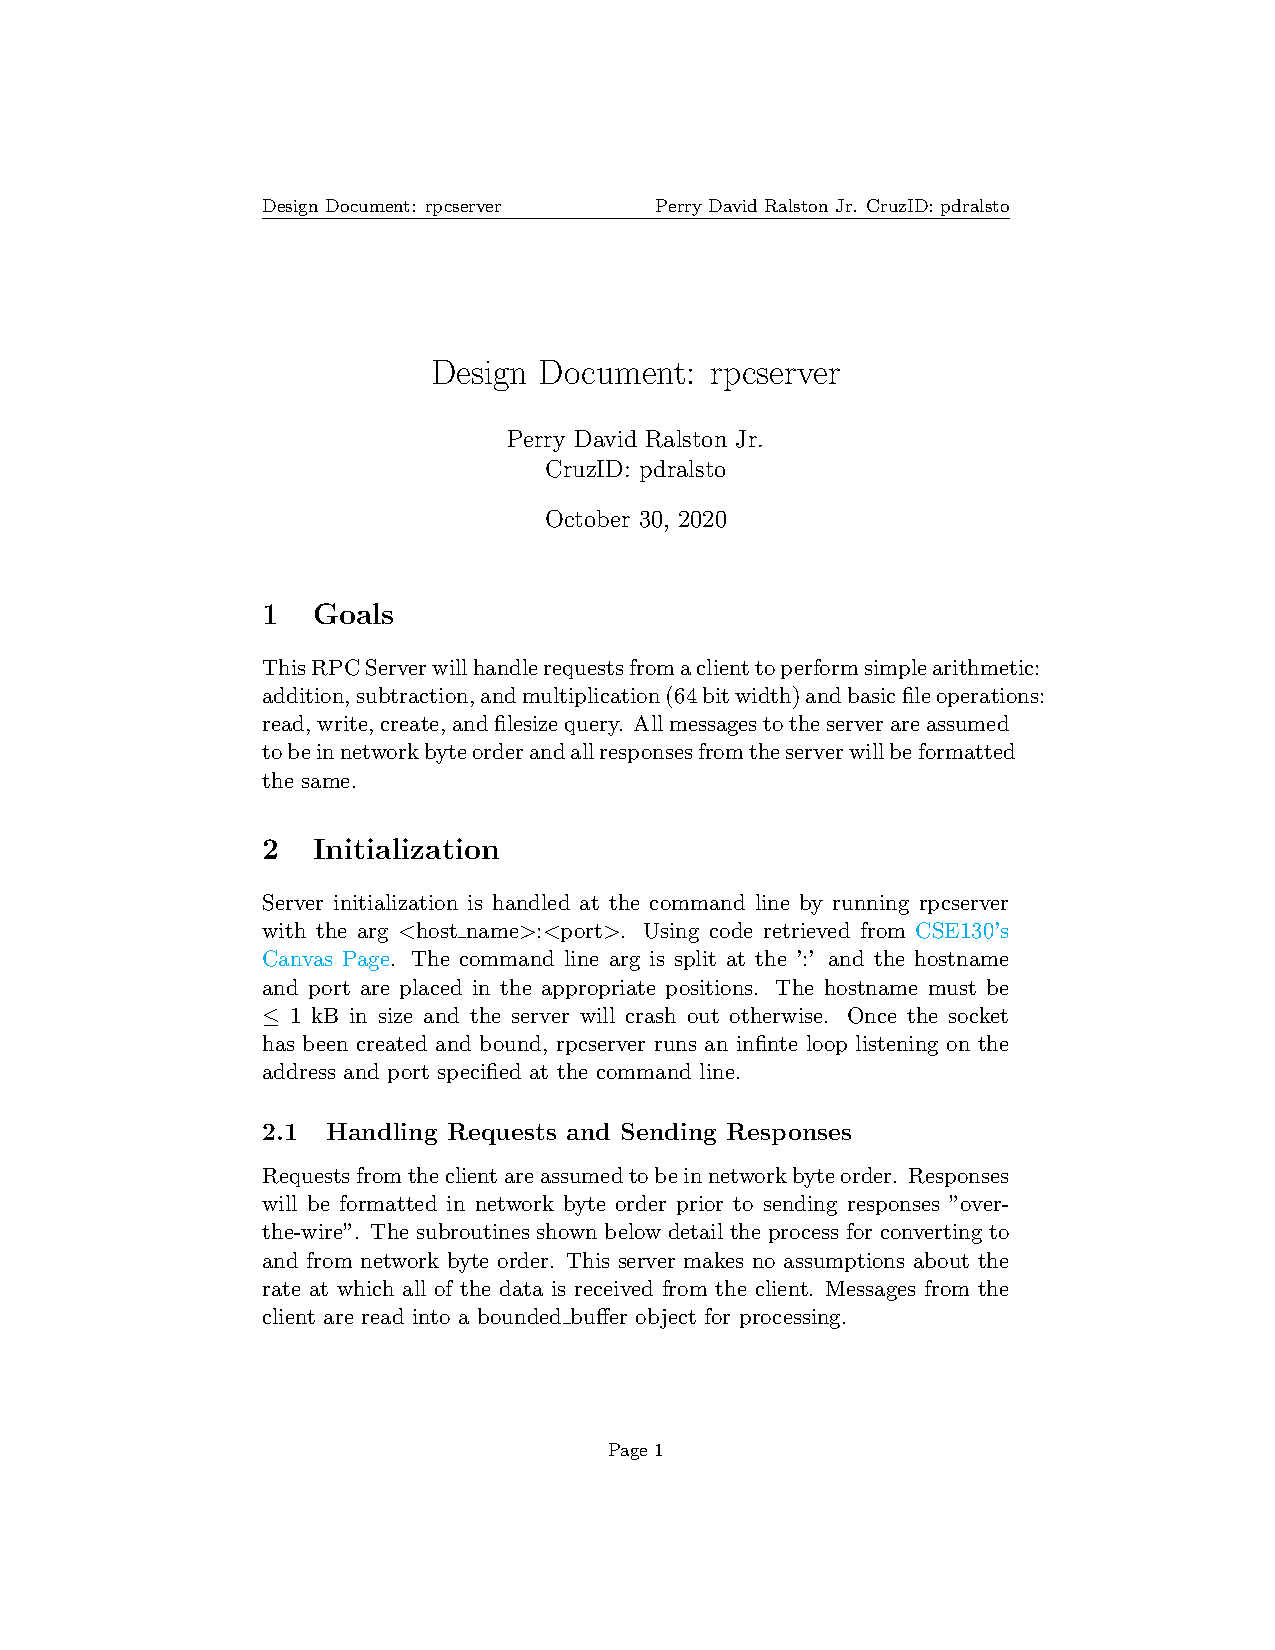
\includepdf[pages={-}]{resources/PREV_DESIGN.pdf}
\end{document}